\documentclass[12pt]{article}
	
%______________________PREAMBULO_________________________

%----------------------Paquetes--------------------------
\usepackage{amsmath,amssymb,amsfonts,latexsym,cancel} % Paquetes de símbolos adicionales.
\usepackage[spanish,es-tabla]{babel} % Idioma español
\usepackage[utf8]{inputenc} % Paquete que nos permite usar los acentos y otros símbolos, directamente del teclado.
%\usepackage[T1]{fontenc} % Cambia el tipo de letra
%\usepackage{lmodern}
\usepackage{mathpazo}
\usepackage{times} % Tipo de letra Times New Roman
\usepackage{csvsimple}
\usepackage{adjustbox}
\usepackage{graphicx} % Paquete para el manejo de gráficos y figuras en el documento.
\usepackage{geometry} % Permite el manejo de los margenes
\usepackage{fancyhdr} % Permite colocar y manejar el encabezado
\usepackage{pstricks}
\usepackage{multicol}
\usepackage{tocbibind}
\usepackage{multicol}
\usepackage{tabularx}\newcolumntype{Y}{>{\centering\arraybackslash}X}
\usepackage{listings}
\usepackage{xcolor}
\usepackage{csvsimple}
\usepackage{siunitx}
\usepackage{verbatim}
\usepackage{apacite}
%\usepackage{hyperref}
%\usepackage{mathpazo} %fuente palatino
%\usepackage{xcolor}
%\usepackage[shortlabels]{enumitem}
%-------------Paquetes para el formato de las citas-------
\usepackage{float}
\usepackage{cite}
\usepackage{wrapfig}
\usepackage[hyphens]{url}
\usepackage[breaklinks,colorlinks=true,linkcolor=black,citecolor=blue, urlcolor=blue]{hyperref}
\lstset{ %
     language=C,                     % El lenguaje del código
     basicstyle=\ttfamily\footnotesize,  % Estilo básico del código
     keywordstyle=\color{blue},      % Color de las palabras clave
     commentstyle=\color{green},     % Color de los comentarios
     stringstyle=\color{red},        % Color de las cadenas
     numbers=left,                   % Colocar numeración de líneas a la izquierda
     numberstyle=\tiny\color{gray},  % Estilo de los números de línea
     stepnumber=1,                   % Numerar todas las líneas
     breaklines=true,                % Romper líneas largas automáticamente
     frame=single,                   % Colocar un marco alrededor del código
     captionpos=b,                   % Colocar el título del código abajo
}
\sisetup{
     round-mode = places,
     round-precision = 2 % Define el número de decimales que deseas
}
%-----------------------------ayuda de paquetes--------------------

\spanishdecimal{.}

%------------------------Margenes----------------------------

%\newgeometry{bottom = 2.5 cm, top = 2.5 cm, left = 2 cm, right = 2 cm} % Modifica el margen {Abajo, Arriba, Izquierda, Derecha

%----------------------------Interlineado----------------------------------

%\doublespacing
%\onehalfspace
%\singlespace
%\spacing{1.5} % Permite personalisar a gusto
%\setlength{\parskip}{2cm} % Es el espacio entre parrafos

%-----------------------------Sangria---------------------------------------

\setlength{\parindent}{0 cm} % Manipula la sangria
\setlength{\headheight}{14.5pt}

%---------------------Portada------------------

%\title{
%%\begin{figure}[h!]
%		
%%	\centering
%%	
\includegraphics[width=\linewidth]{Nom_UAdeC_FCFM.png}  			
%			
%%\end{figure}
%\huge \textbf{LABORATORIO DE FISICA 3}\\\LARGE TITULO PRACTICA\\}
%\author{ \Large \textbf{Profesor:}\\
%\Large \textbf{Alumno:} Oscar Joel Castro Contreras}
%\date{\today}

%--------------Encabezado y pie de pagina--------------------

\pagestyle{fancy}%Coloca el encabezado en el documento
\lhead[]{Física Moderna}%Encabezado izquierda
\rhead[]{Oscar Joel Castro Contreras}%Encabesado derecha
%\chead[]{}%Encabesado central
\renewcommand{\headrulewidth}{0.08 pt}%Coloca linea al pie de pagina

%\lfoot[]{PI}%Pie de pagina izquerdo
%\rfoot[]{PD}%Pie de pagina derecho
\cfoot[]{\thepage}%Pie de pagina central
\renewcommand{\footrulewidth}{0.08 pt}%Coloca linea al pie de pagina

%-----------------------------------------------------------------------------

\begin{document}
	
	\begin{titlepage}
	
		\centering
		{\bfseries
               {\scshape\LARGE Tabla Periodica \par}
		\par}
		%\vspace{1cm} 
		%{\LARGE Ensayo Tema 7\par}
		\vspace{1cm}
		{\LARGE \textbf{Oscar Joel Castro Contreras} \par}
          \vspace{0.5cm}
          {\large Cursos Propedéuticos Maestría En Ciencias Físicas\par}
          {\large Materia: Física Moderna\par}
		\vspace{1cm}
           
          %\vfill
          {\large (IFUAP Instituto de Física De La Universidad Autónoma De Puebla) \par}
		{\large (\Today) \par}
		\thispagestyle{empty}
		%\thispagestyle{fancy}
          \vspace{1cm}

	\end{titlepage}

     \newpage

     \thispagestyle{empty}

     \begingroup
     
     \renewcommand{\addtocontents}[2]{}
	
     \tableofcontents		
	
     \endgroup
	
     \newpage
     
	\pagenumbering{arabic}
     \setcounter{page}{1} 
	
     \section{Introducción}\label{sec:Introducción}

          \subsection{Antecedentes históricos}\label{sec:Antecedentes históricos}
               La Tabla Periódica es una obra colectiva, en continuo crecimiento y, sobre todo, una herramienta fundamental, permite explicar, conocer y anticipar las propiedades de la materia.\\\\
               Como desde el principio se comprobó la existencia de familias de elementos que presentaban muchas semejanzas entre sí, se intuyó que debía de existir una ley natural que los relacionase y agrupase. La búsqueda de esta ley natural está plagada de numerosos intentos, basados, por lo general, en dos criterios fundamentales:
               
               \begin{itemize}
                    \item La semejanza de las propiedades físicas y químicas de los elementos y sus compuestos.
                    \item La relación que estas propiedades pudieran tener con alguna característica de los átomos, principalmente con la masa atómica.
               \end{itemize}

               La figura de Mendeléiev y de otros grandes científicos nos permite indicar como la enseñanza fue motor de las clasificaciones que surgieron en la segunda mitad del siglo XIX.\\\\
               La Tabla Periódica de Mendeléiev ha tenido tal impacto científico y cultural que se pensó que se trataba de una obra prácticamente acabada. Tras 150 años podemos celebrar sus numerosos éxitos incorporando algunos elementos, la mayoría obtenidos sintéticamente.
             
               \subsection{Cronología}\label{sec:Cronología}
                    \subsubsection{Antoine-Laurent de Lavoisier (1743-1794)}\label{sec:Antoine-Laurent de Lavoisier (1743-1794)}
                         Autor del primer texto de química moderno, “Método de nomenclatura química” (1787), por la nomenclatura que desarrolla para los compuestos y los elementos, con lo que se consiguió prescindir de la terminología alquímica que se utilizaba.\\
                         Su libro “Tabla de los compuestos elementales” (1789) clasificó los treinta y tres elementos conocidos en su tiempo, en no metales, formadores de ácidos, y en metales, formadores de sales.
                    
                    \subsubsection{Jacob Berzelius (1779-1848)}\label{sec:Jacob Berzelius (1779-1848)}
                         Implantó el sistema de símbolos químicos que existe en la actualidad, y mantuvo la clasificación de Lavoisier basándose en el aspecto y en las propiedades físicas de los elementos. Descubrió algunos elementos como cerio, selenio y torio, y consiguió aislar silicio, circonio y titanio.

                    \subsubsection{Joham W. Döbereiner (1780-1849)}\label{sec:Joham W. Döbereiner (1780-1849)}
                         Observó que ciertas agrupaciones de tres elementos presentaban propiedades muy parecidas, y les denominó triadas. En tales triadas el peso atómico del elemento central era aproximadamente la media aritmética del peso atómico de los elementos extremos.
                    
                    \subsubsection{Alexandre-Emile Béguyer de Chancourtois (1820 –1886)}\label{sec:Alexandre-Emile Béguyer de Chancourtois (1820 –1886)}
                         Propuso una clasificación de los elementos químicos colocándolos sobre la superficie de un cilindro (tornillo telúrico). Los elementos se disponían sobre una línea diagonal formando un ángulo de 45 º con la horizontal, dibujando una espiral y estaban ordenados según su peso atómico creciente (expresados en números enteros),de manera que los que tenían propiedades parecidas se situaban en una misma línea vertical, denominada generatriz del cilindro.
                    
                    \subsubsection{John Alexander Reina Newlands (1837-1898)}\label{sec:John Alexander Reina Newlands (1837-1898)}
                         Precursor en la elaboración del sistema periódico de los elementos, estableció la ley de recurrencia en 1864, que condujo a establecer la llamada ley de las octavas: Ordenando los elementos en orden creciente con respecto a su peso atómico, el octavo elemento tiene propiedades muy parecidas al primero; el noveno al segundo; etc., igual que ocurre con las notas de la escala musical. Esta ley no pudo aplicarse a elementos de peso atómico superior al del calcio.

                    \subsubsection{Julius Lothar Meyer (1830 – 1895)}\label{sec:Julius Lothar Meyer (1830 – 1895)}
                         Puso de relevancia que existía una cierta periodicidad en el volumen atómico.\\
                         En función del volumen atómico y de otras propiedades como el peso atómico, Lothar Meyer construyó una Tabla Periódica en la que aparecen ordenados los elementos según el peso atómico creciente, semejante a la de Mendeleiev.\\
                         En la tabla de Lothar Meyer, en posiciones horizontales, los elementos aparecen ordenados de forma similar a los actuales grupos; y en posiciones verticales, aparecen los elementos correspondientes a los actuales periodos.

               \subsection{Tabla Periódica de Mendeleiev}\label{sec:Tabla Periódica de Mendeleiev}
               En 1869 y 1870, dos científicos, el ruso D. Mendeleiev (1834-1907) y el alemán L. Meyer (1830-1895), presentaron independientemente su célebre Tabla Periódica.\\\\
               La clasificación periódica de Mendeleiev, más elaborada que la de Meyer, contenía todos los elementos conocidos hasta entonces, ordenados en una tabla de doble entrada según los criterios siguientes:

               \begin{itemize}
                    \item Masa atómica creciente. Los elementos se ordenan de izquierda a derecha, según este criterio, en líneas horizontales.
                    \item Semejanza en las propiedades. Los elementos que presentan pro piedades semejantes se sitúan en columnas verticales.
               \end{itemize}

               El planteamiento de Mendeleiev fue que las propiedades de los elementos debían responder a una ley periódica que todavía se desconocía.\\\\
               Ese convencimiento le llevó a predicciones arriesgadas, que el tiempo confirmó como ciertas:

               \begin{itemize}
                    \item Cuestionar el valor de la masa atómica de algunos elementos, como el indio, el berilio y el uranio, y asignarles otro valor que consideró más correcto.
                    \item Invertir el orden de masas atómicas en ciertos elementos para que éstos quedasen agrupados con otros de sus mismas propiedades, como teluro-yodo o cobalto-níquel.
                    \item Dejar huecos en la tabla correspondientes a elementos aún no des cubiertos y predecir las propiedades que tendrían. Es el caso del galio, el germanio o el escandio.
               \end{itemize}

               La clasificación propuesta por Mendeleiev y Meyer experimentó diversas modificaciones con el paso del tiempo, pero pese a ello, mantenía una sustancial dificultad: considerar la masa atómica como el criterio de ordenación implica colocar varios elementos fuera de su lugar para que queden agrupados por semejanza de propiedades.\\\\
               Por lo tanto, había que compatibilizar los dos hechos: las propiedades químicas de los elementos se repiten periódicamente y la masa atómica no es criterio suficiente para obtener una ordenación coherente.

          \subsection{Sistema periódico actual}\label{sec:Sistema periódico actual}
               La propiedad fundamental en que se basa la ley periódica se respondio hasta que en 1914 H. Moseley (1887-1915) determinó el número atómico de los elementos y comprobó que si se colocaban los elementos por orden creciente de su número atómico, todos quedaban situados en el lugar requerido por el criterio de semejanza de propiedades.\\\\
               Se estructuró en 18 Grupos o columnas y 7 Periodos o filas. Esta estructura fue propuesta por el químico suizo Alfred Werner (1866 - 1919; Premio Nobel de Química en 1913) y por el químico austriaco Friedrich Adolf Paneth (1887 – 1958).
               
          \subsection{Ley periódica}\label{sec:Ley periódica}
               La ley periódica se enuncia así en la actualidad:

               \begin{center}
                    \textit{Cuando los elementos se colocan en orden creciente de su número atómico, tiene lugar una repetición periódica de ciertas propiedades físicas o químicas de aquéllos.}
               \end{center}

               El origen de la periodicidad en las propiedades químicas de los elementos radica en la configuración de sus electrones más externos o electrones de valencia, y ésta se repite periódicamente.
          
          \section{Desarrollo}\label{sec:Desarrollo}
               
               \subsection{Estructura del sistema periódico}\label{sec:Estructura del sistema periódico}
                    La actual Tabla Periódica se debe a Paneth y Werner. En ella los 109 elementos conocidos hasta el momento están clasificados en orden creciente de su número atómico en dieciocho columnas y siete filas. Las filas reciben el nombre de períodos y las columnas, de grupos.\\\\
                    En cada grupo se colocan los elementos de propiedades análogas, y cada período se construye colocando elementos que aumentan en una unidad el número atómico del elemento precedente.\\\\
                    Esta ordenación se realiza extendiendo los períodos largos de Mendeleiev, evitando así que aparezcan mezclados elementos metálicos y no metálicos, y que la distribución electrónica periódica, principal responsable de sus propiedades, sea más coherente.\\\\
                    La distribución de familias de elementos en el sistema periódico es:

                    \begin{itemize}
                         \item \textbf{Elementos representativos} formados por:
                    \end{itemize}
                    \begin{flushright}
                         \begin{tabular}{rl}
                              Alcalinos:               & Grupo IA \\
                              Alcalinotérreos:         & Grupo IIA \\
                              Térreos o Boroideos:     & Grupo IIIA \\
                              Carbonoideos:            & Grupo IVA \\
                              Nitrogenoideos:          & Grupo VA \\
                              Anfígenos:               & Grupo VIA \\
                              Halógenos:               & Grupo VIIA \\
                              Gases nobles o inertes:  & Grupo VIIIA, también llamado 0
                         \end{tabular}
                    \end{flushright}

                    
                    \begin{itemize}
                         \item \textbf{Elementos de transición} formados por los grupos IIIB, IVB, VB, VIB, VIIB, VIIIB (que incluye tres columnas), IB y IIB. Se sitúan en el centro del Sistema Periódico.
                         \item \textbf{Elementos de transición interna} formados por las familias de Lantánidos y Actínidos, de 14 elementos cada una. Se colocan en dos filas habitualmente fuera del entorno general.
                         \item El \textbf{hidrógeno} queda fuera de estas consideraciones, y por tener un solo electrón que está alojado en el orbital 1s, suele colocarse encima del grupo de Alcalinos IA.
                    \end{itemize}

                    La Tabla Periódica que utilizamos hoy en día se estructura según la con figuración electrónica de los elementos. Esta es la responsable de las propiedades de éstos.

               \subsection{Períodos}\label{sec:Períodos}
                    Los períodos se designan por números correlativos del 1 al 7. En ellos los elementos presentan propiedades diferentes que varían progresiva mente desde el comportamiento metálico hasta el comportamiento no metálico, para acabar siempre con un gas noble.\\\\
                    El nivel energético en el que se encuentran los electrones de valencia en los elementos de un período dado es el mismo, ya que uno posee un electrón de valencia más que el anterior. Este electrón recibe el nombre de electrón diferenciador y es el responsable de la diferencia entre las propiedades de elementos correlativos en un período.\\\\
                    Observe que los elementos del mismo período tienen sus electrones más internos ordenados como el gas noble del período anterior. Reciben el nombre de estructura interna, y es habitual abreviar la configuración electrónica sustituyendo la estructura interna por el símbolo del gas noble, entre corchetes, seguido de la configuración electrónica de los electrones de valencia.\\\\
                    Los elementos de un período determinado se caracterizan por tener electrones en el mismo nivel más externo, que es precisamente el número que designa cada período. Así, los elementos del período 1 tienen electrones sólo en el nivel 1, los del período 2 tienen electrones ocupando hasta el nivel 2, los del tercer período tienen electrones hasta el nivel 3, y así sucesivamente.\\\\
                    Por ejemplo, los elementos del tercer período tienen todos estructura interna de neón y sus electrones ocupan hasta el tercer nivel.
                    \begin{center}
                         \begin{tabular}{llllcllll}
                              Na&(Z=11)&→&[Ne]$ 3s^1      $&     &P &(Z=13)&→&[Ne] $3s^2 3p^3 $ \\
                              Mg&(Z=12)&→&[Ne]$ 3s^2      $&     &S &(Z=14)&→&[Ne] $3s^2 3p^4 $ \\
                              Al&(Z=13)&→&[Ne]$ 3s^2 3p^1 $&     &Cl&(Z=15)&→&[Ne] $3s^2 3p^5 $\\ 
                              Si&(Z=14)&→&[Ne]$ 3s^2 3p^2 $&     &Ar&(Z=16)&→&[Ne] $3s^2 3p^6 $ \\
                         \end{tabular}
                    \end{center}
               
               \subsection{Grupos}\label{sec:Grupos}
                    Los grupos se designan mediante números correlativos del 1 al 18.\\\\
                    Los elementos que componen cada grupo tienen, con escasas excepciones, similares propiedades químicas, debido a que todos coinciden en su configuración electrónica de los electrones de valencia.

                    \begin{itemize}
                         \item Los grupos 1 y 2 corresponden a los elementos metálicos.
                         \item Los metales de transición ocupan los grupos 3 al 12.
                         \item Los no metales y los semimetales ocupan los grupos 13 al 17.
                         \item El grupo 18 está constituido por los gases nobles.
                    \end{itemize}

                    Los grupos 1, 2 y del 13 al 18 están constituidos por los elementos que se conocen como elementos representativos. Algunos de estos grupos reciben nombres especiales:

                    \begin{table}[H]
                         \centering
                         \begin{adjustbox}{max width=\textwidth}
                              \csvautotabular{g_c_e_r.csv}
                         \end{adjustbox}
                         %\caption{Tabla de los grupos con los elementos representativos.}
                         \label{tab:1}
                    \end{table}

                    Entre los metales de transición se encuentran los elementos conocidos como tierras raras o metales de transición interna: lantánidos y actínidos, que suelen escribirse aparte en dos filas de catorce columnas.\\\\
                    En los elementos de transición, el electrón diferenciador ocupa un orbital d, y en los de transición interna, un orbital f. La configuración electrónica de estos grupos de elementos no es tan regular como en los elementos representativos y son frecuentes las excepciones.\\\\
                    Observe que el número de columnas en la Tabla Periódica está directamente relacionado con el número de electrones que caben en cada subnivel.
                    
                    \begin{table}[H]
                         \centering
                         \begin{adjustbox}{max width=\textwidth}
                              \csvautotabular{g_m_y_nm.csv}
                         \end{adjustbox}
                         %\caption{Tabla de los grupos y sus capacidades en cada subnivel.}
                         \label{tab:2}
                    \end{table}

               \subsection{Propiedades periódicas de los elementos}\label{sec:Propiedades periódicas de los elementos}
                    Ya sabemos que algunas propiedades físicas y químicas se repiten con cierta regularidad a lo largo de los grupos y los períodos.\\\\
                    La razón de su regularidad reside en la configuración electrónica y en el número atómico del elemento. La carga nuclear efectiva sobre el electrón más externo reúne estas dos características y facilita el estudio de la variación de las propiedades periódicas de los elementos al aumentar su número atómico.\\\\
                    Las propiedades periódicas más importantes son: el radio atómico y el radio iónico, la energía de ionización, la afinidad electrónica, la electro negatividad y el carácter metálico.

                    \begin{figure}[H]
                         \centering
                         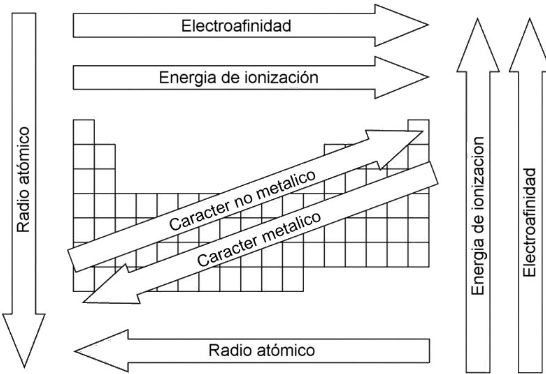
\includegraphics[height=5cm]{Propiedades_Periodicas.png}
                         %caption{Resumen de las propiedades periódicas.}
                         \label{Fig:One-hot_endcoding_AF01}
                    \end{figure}
               
     %\begin{thebibliography}{8}
     %     \bibitem{ref_1}
     %     Fontes, L. M. A. M. D. S. (2023). Scaleddown EfficientNet for Facial Expression Recognition (Doctoral dissertation). \href{http://hdl.handle.net/10400.6/14202}{http://hdl.handle.net/10400.6/14202}
     %     \bibitem{ref_2}
     %     Fritz. (2023, 18 septiembre). Reviewing EfficientNet: Increasing the Accuracy and Robustness of CNNs. Fritz Ai. \href{https://fritz.ai/efficientnet-review/}{https://fritz.ai/efficientnet-review/}
     %     \bibitem{ref_3}
     %     Tan, M., \& Le, Q., V. (2019, 28 mayo). EfficientNet: Rethinking Model Scaling for Convolutional Neural Networks. arXiv.org. \href{https://arxiv.org/abs/1905.11946}{https://arxiv.org/abs/1905.11946}
     %     \bibitem{ref_4}
     %     Lundqvist, D., Flykt, A., \& Öhman, A. (1998). The Karolinska Directed Emotional Faces - KDEF, CD ROM from Department of Clinical Neuroscience, Psychology section, Karolinska Institutet, ISBN 91-630-7164-9. \href{https://kdef.se/}{https://kdef.se/}
     %     \bibitem{ref_5}
     %     Seger, C. (2018). An investigation of categorical variable encoding techniques in machine learning: binary versus one-hot and feature hashing. \href{https://urn.kb.se/resolve-?urn=urn-%3Anbn-%3Ase-%3Akth-%3Adiva-237426}{https://urn.kb.se/resolve?-urn=urn-\%3Anbn-\%3Ase-\%3Akth-\%3Adiva-237426}
     %     
     %\end{thebibliography}
     
     \nocite{*}
     \bibliographystyle{apacite}    
     \bibliography{referencias_tema7}

\end{document}